
%%%%%%%%%%%%%%%%%%%%%%%%%%%%%%%%%%%%%%%%%%%%%%%%%%%%%%%%%%%%%%%%%%%%%
%
% Axel Fahy
% 10.01.2016
% Eshop
%
%%%%%%%%%%%%%%%%%%%%%%%%%%%%%%%%%%%%%%%%%%%%%%%%%%%%%%%%%%%%%%%%%%%%%%

\documentclass[12pt]{article}
\usepackage[a4paper]{geometry}
\usepackage[utf8]{inputenc}
\usepackage[myheadings]{fullpage}
\usepackage{fancyhdr}
\usepackage{lastpage}
\usepackage{graphicx, wrapfig, subcaption, setspace, booktabs}
\usepackage[T1]{fontenc}
\usepackage[font=small, labelfont=bf]{caption}
\usepackage{fourier}
\usepackage[protrusion=true, expansion=true]{microtype}
\usepackage[english]{babel}
\usepackage{sectsty}
\usepackage{url, lipsum}
\usepackage{parskip}                                                  % Remove identation
\usepackage{caption}
\usepackage{hhline}

% Tables alignement with fix sized
\usepackage{array}
\newcolumntype{L}[1]{>{\raggedright\let\newline\\\arraybackslash\hspace{0pt}}m{#1}}
\newcolumntype{C}[1]{>{\centering\let\newline\\\arraybackslash\hspace{0pt}}m{#1}}
\newcolumntype{R}[1]{>{\raggedleft\let\newline\\\arraybackslash\hspace{0pt}}m{#1}}


%-------------------------------------------------------------------------------
% USE CASE FORMAT
%-------------------------------------------------------------------------------
\usepackage{booktabs}
\newcommand\addrow[2]{#1 &#2\\ }

\newcommand\addheading[2]{\textbf{#1} &#2\\ \hline}
\newcommand\tabularhead{\begin{tabular}{lp{11cm}}
\hline
}

\newcommand\addmulrow[2]{ \begin{minipage}[t][][t]{3.5cm}#1\end{minipage}%
    &\begin{minipage}[t][][t]{11cm}
    \begin{enumerate} #2   \end{enumerate}
    \end{minipage}\\ }

\newenvironment{usecase}{\tabularhead}
{\hline\end{tabular}}


%-------------------------------------------------------------------------------
% CODE FORMAT
%-------------------------------------------------------------------------------
\usepackage{listings}                                                 % Code listings
\usepackage{listingsutf8}
\lstset{inputencoding=utf8/latin1}
\usepackage{color}
\definecolor{mygreen}{rgb}{0,0.6,0}
\definecolor{mygray}{rgb}{0.5,0.5,0.5}
\definecolor{mymauve}{rgb}{0.58,0,0.82}
\definecolor{bggray}{rgb}{0.95, 0.95, 0.95}
\lstset{ %
    %backgroundcolor=\color{bggray},   % choose the background color; you must add \usepackage{color} or \usepackage{xcolor}
    basicstyle=\footnotesize,        % the size of the fonts that are used for the code
    breakatwhitespace=false,         % sets if automatic breaks should only happen at whitespace
    breaklines=true,                 % sets automatic line breaking
    captionpos=b,                    % sets the caption-position to bottom
    %commentstyle=\color{mygreen},    % comment style
    deletekeywords={...},            % if you want to delete keywords from the given language
    escapeinside={\%*}{*)},          % if you want to add LaTeX within your code
    extendedchars=true,              % lets you use non-ASCII characters; for 8-bits encodings only, does not work with UTF-8
    frame=none,                    % adds a frame around the code
    frameround=tttt                  % tttt for having the corner round.
    keepspaces=true,                 % keeps spaces in text, useful for keeping indentation of code (possibly needs columns=flexible)
    keywordstyle=\color{blue},       % keyword style
    language=html,                 % the language of the code
    morekeywords={*,...},            % if you want to add more keywords to the set
    numbers=none,                    % where to put the line-numbers; possible values are (none, left, right)
    numbersep=5pt,                   % how far the line-numbers are from the code
    numberstyle=\tiny\color{mygray}, % the style that is used for the line-numbers
    rulecolor=\color{black},         % if not set, the frame-color may be changed on line-breaks within not-black text (e.g. comments (green here))
    showspaces=false,                % show spaces everywhere adding particular underscores; it overrides 'showstringspaces'
    showstringspaces=false,          % underline spaces within strings only
    showtabs=false,                  % show tabs within strings adding particular underscores
    stepnumber=1,                    % the step between two line-numbers. If it's 1, each line will be numbered
    %stringstyle=\color{mymauve},     % string literal style
    tabsize=2,                       % sets default tabsize to 2 spaces
    %title=\lstname                   % show the filename of files included with \lstinputlisting; also try caption instead of title
}


\newcommand{\HRule}[1]{\rule{\linewidth}{#1}}
\onehalfspacing
\setcounter{tocdepth}{5}
\setcounter{secnumdepth}{5}


% Remove the 'Chapter' before each chapter.
%\usepackage{titlesec}
%\titleformat{\chapter}{}{}{0em}{\bf\LARGE}

%\makeatletter
%\renewcommand{\@makechapterhead}[1]{%
%\vspace*{0 pt}%
%\bfseries\Huge\thechapter.\ #1
%\par\nobreak\vspace{40 pt}}}
%\makeatother

%-------------------------------------------------------------------------------
% HEADER & FOOTER
%-------------------------------------------------------------------------------
\pagestyle{fancy}
\fancyhf{}
\setlength\headheight{15pt}
\fancyhead[L]{}
\fancyhead[R]{\textsl{EShop}}
\fancyfoot[R]{\textsl{Page \thepage\ of \pageref{LastPage}}}

%-------------------------------------------------------------------------------
% TITLE PAGE
%-------------------------------------------------------------------------------
\begin{document}

\title{ \normalsize \textsc{Projet logiciel}
        \\ [2.0cm]
        \HRule{0.5pt} \\
        \LARGE \textbf{\uppercase{EShop}}
        \HRule{2pt} \\ [0.5cm]
        \normalsize \today \vspace*{5\baselineskip}}

\date{}

\author{
    Axel Fahy / Rudolf Höhn / Benjamin Ganty / Robin Chappatte / Pierre-Yves Kugler\\
    hepia - ITI}

\clearpage
\maketitle
\thispagestyle{empty} % Remove the number on page title.
\newpage
\tableofcontents
\newpage

%-------------------------------------------------------------------------------
% Section title formatting
\sectionfont{\scshape}
%-------------------------------------------------------------------------------

%-------------------------------------------------------------------------------
% BODY
%-------------------------------------------------------------------------------

\section{\textit{User Stories}}

\begin{center}
    \begin{tabular}{ | L{13cm} || C{2cm} | }
        \hline
        \textbf{Description} & \textbf{Priorité}\\
        \hhline{|=||=|}
        Le client veut voir les produits du magasin & 1\\
        \hline
        Le client veut avoir la description du produit en cliquant dessus & 2\\
        \hline
        Le client va voir dans le rayon d'à cote les produits proposés & 3\\
        \hline
        Le client veut pouvoir filtrer les produits par catégories & 4\\
        \hline
        Le client veut revenir au choix des catégories & 5\\
        \hline
        Le client ne trouve pas le produit qu'il cherche et demande a un employe du magasin de l'aider & 6\\
        \hline
        Le client dans le magasin veut ramasser un produit sur une étagere et le mettre dans son panier & 7\\
        \hline
        Le client veut voir son panier & 8\\
        \hline
        Le client n'est pas content avec un de ses articles dans le panier et souhaite le retirer & 9\\
        \hline
        Le client veut modifier la quantité d'un element situé dans le panier & 10\\
        \hline
        Le client veut vider son panier & 11\\
        \hline
        Le client veut supprimer un element du panier & 12\\
        \hline
        Le client veut connaitre le solde total de son panier & 13\\
        \hline
        Le client avec son panier veut pouvoir aller à la caisse et va payer ses courses & 14\\
        \hline
        Le client veut rentrer ses informations de paiement et payer & 15\\
        \hline
        Le client veut se créer un compte & 16\\
        \hline
        Le client veut payer mais il doit d'abord s'authentifier & 17\\
        \hline
        Le client veut modifier son compte (nom, mot de passe, adresse) & 18\\
        \hline
        Le client veut supprimer son compte & 19\\
        \hline
        Le client veut se déconnecter de son compte & 20\\
        \hline
    \end{tabular}
\end{center}

\newpage
\section{\textit{Use case}}

\subsection{Diagramme}

\begin{figure}[ht]
    \center
    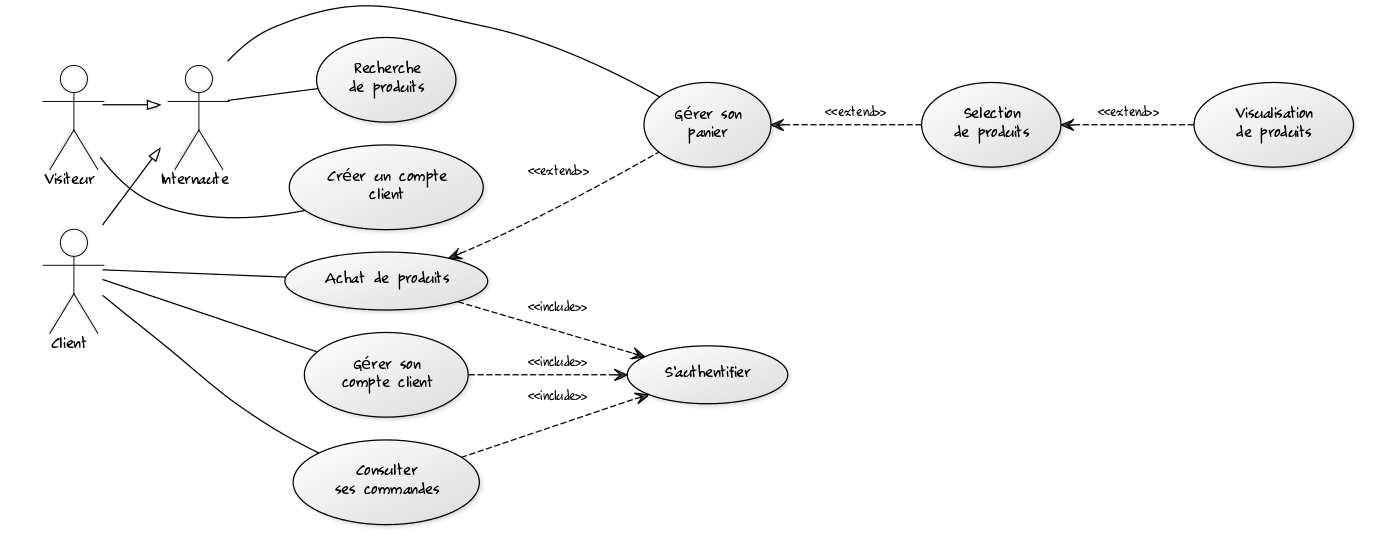
\includegraphics[scale=0.33]{../Diagrams/UseCaseDiagrams/usecase_global.png}
    \caption*{Diagramme UML des \textit{use case}}
\end{figure}

\subsection{Détails}

\begin{usecase}
    \addheading{Titre}{Visualisation des produits}
    \addrow{Acteur}{Client}
    \addrow{But}{Permettre au client de connaître les produits à disposition.}
    \addrow{Pré-condition}{Le client accède à l'application web et voit les produits.}
    \addrow{Scénario alternatif}{Le client recherche un article en particulier.}
    \addrow{Exception}{Il n'y a pas de produit disponible.}
\end{usecase}

\begin{usecase}
    \addheading{Titre}{Sélection de produits}
    \addrow{Acteur}{Client}
    \addrow{But}{Permettre au client de sélectionner des produits.}
    \addrow{Résumé métier}{Le client doit pouvoir séléctionner le(s) produit(s) à acheter et les mettre dans son panier.}
    \addrow{Pré-condition}{Le client doit être authentifié.}
\end{usecase}

\begin{usecase}
    \addheading{Titre}{Achat de produits}
    \addrow{Acteur}{Client}
    \addrow{But}{Permettre au client d'acheter des produits.}
    \addrow{Résumé métier}{Le client doit pouvoir séléctionner le(s) produit(s) à acheter.}
    \addmulrow{Pré-conditions}{
    \item Le client doit être authentifié.
    \item Les produits doivent être disponibles.
    }
    \addmulrow{Scénario alternatif}{
    \item Acheter plusieurs produits d'un coup.
    \item Avoir plusieurs fois le même produit.
    }
    \addmulrow{Exception}{
    \item Les produits ne sont pas en stock.
    }
\end{usecase}

\begin{usecase}
    \addheading{Titre}{Gestion de panier}
    \addrow{Acteur}{Client}
    \addrow{But}{Permettre au client de modifier, supprimer un élément du panier}
    \addrow{Résumé métier}{Le client doit pouvoir modifier la quantité d'un élément de son panier et de le supprimer}
    \addrow{Pré-condition}{Avoir des produits dans son panier}
\end{usecase}

\begin{usecase}
    \addheading{Titre}{Gestion de son compte client}
    \addrow{Acteur}{Client}
    \addrow{But}{Permettre au client de modifier, supprimer son compte}
    \addrow{Résumé métier}{Le client doit pouvoir modifier ses informations de facturations, de paiements ou de supprimer son compte}
    \addrow{Pré-condition}{Etre authentifié}
\end{usecase}

\begin{usecase}
    \addheading{Titre}{Consultation des commandes}
    \addrow{Acteur}{Client}
    \addrow{But}{Permettre au client de voir ses commandes en cours}
    \addrow{Résumé métier}{Le client doit pouvoir voir l'état de ses commandes}
    \addrow{Pré-condition}{Etre authentifié}
\end{usecase}

\newpage
\section{Maquettes}

Voici les différents écrans de l'applicaiton.

\subsection{Inscription}

\begin{figure}[ht]
    \center
    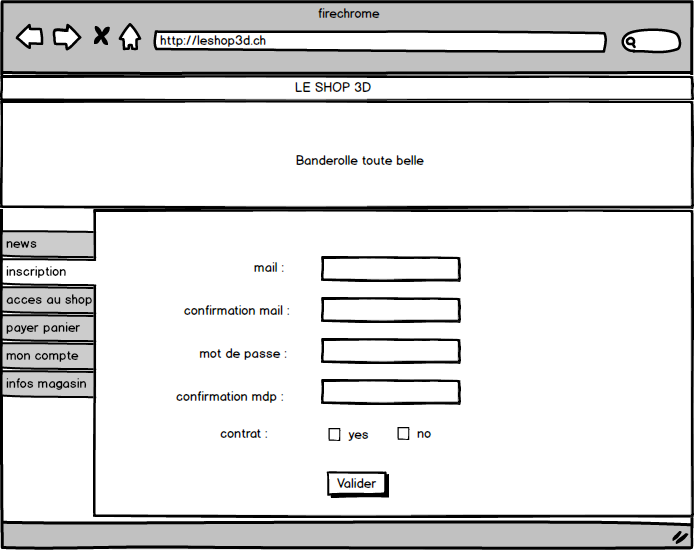
\includegraphics[scale=0.6]{../Maquettes/inscription.jpeg}
    \caption*{Inscription dans le EShop}
\end{figure}

\newpage
\subsection{Page d'accueil}

\begin{figure}[ht]
    \center
    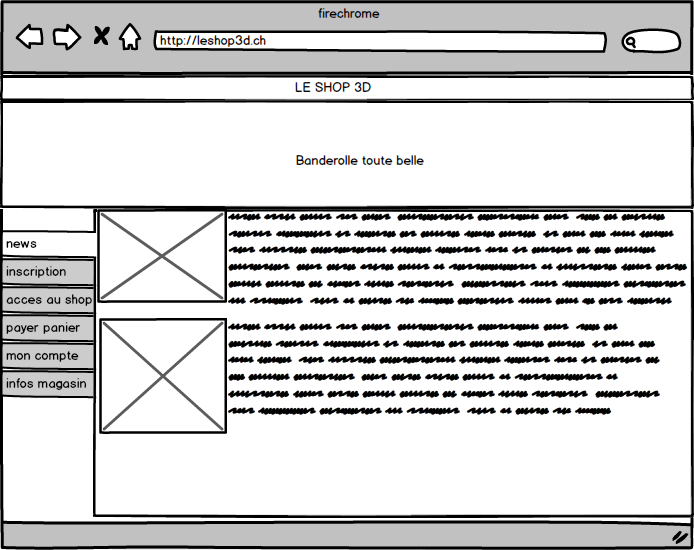
\includegraphics[scale=0.6]{../Maquettes/page_accueil.jpeg}
    \caption*{Page d'accueil du EShop}
\end{figure}

\newpage
\subsection{Visualisation du panier}

\begin{figure}[ht]
    \center
    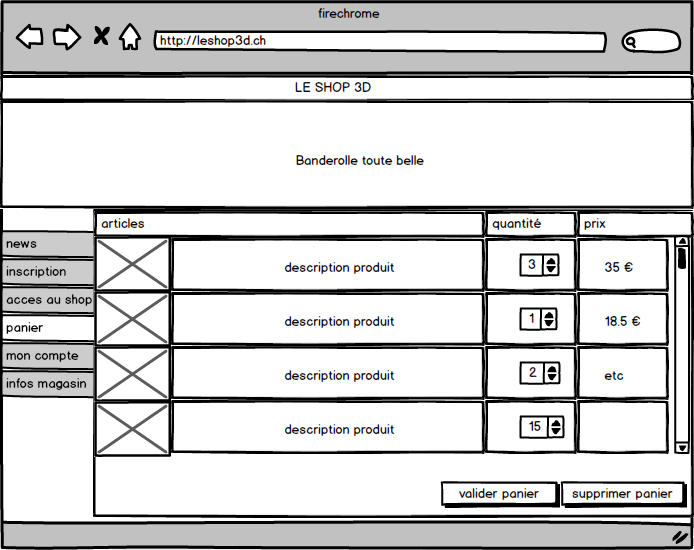
\includegraphics[scale=0.6]{../Maquettes/visualisation_panier.jpeg}
    \caption*{Visualisation du panier du EShop}
\end{figure}

\newpage
\subsection{Compte client}

\begin{figure}[ht]
    \center
    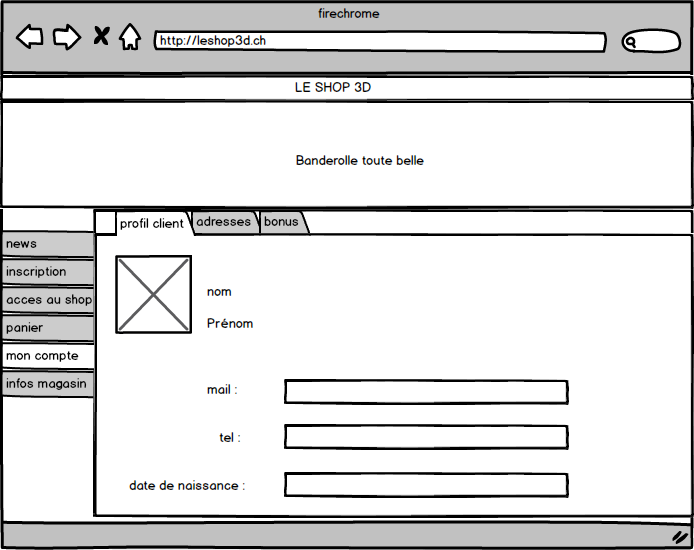
\includegraphics[scale=0.6]{../Maquettes/compte_client.jpeg}
    \caption*{Compte client du EShop}
\end{figure}

\newpage
\subsection{Informations client}

\begin{figure}[ht]
    \center
    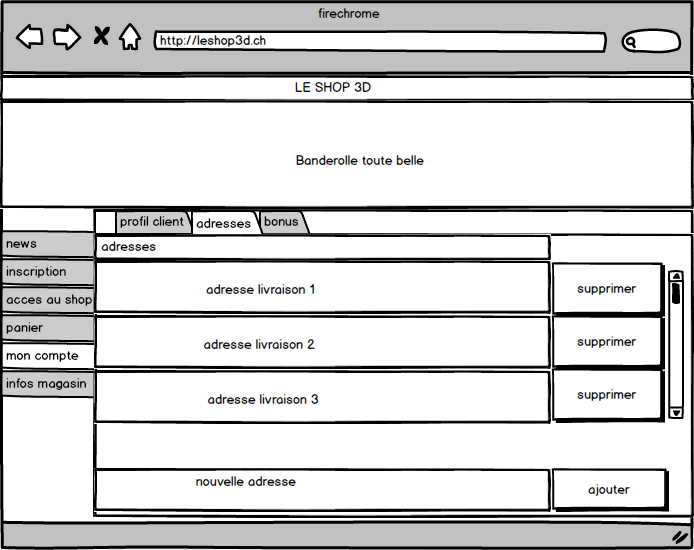
\includegraphics[scale=0.6]{../Maquettes/compte_client_adresse.jpeg}
    \caption*{Information du client du EShop}
\end{figure}

\newpage
\subsection{Règlement à domicile}

\begin{figure}[ht]
    \center
    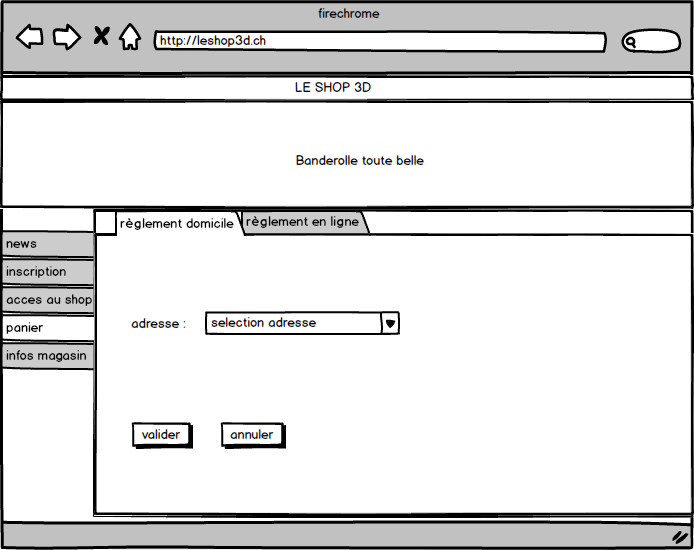
\includegraphics[scale=0.6]{../Maquettes/reglement_domicile.jpeg}
    \caption*{Règlement à domicile de la commande}
\end{figure}

\newpage
\subsection{Règlement online}

\begin{figure}[ht]
    \center
    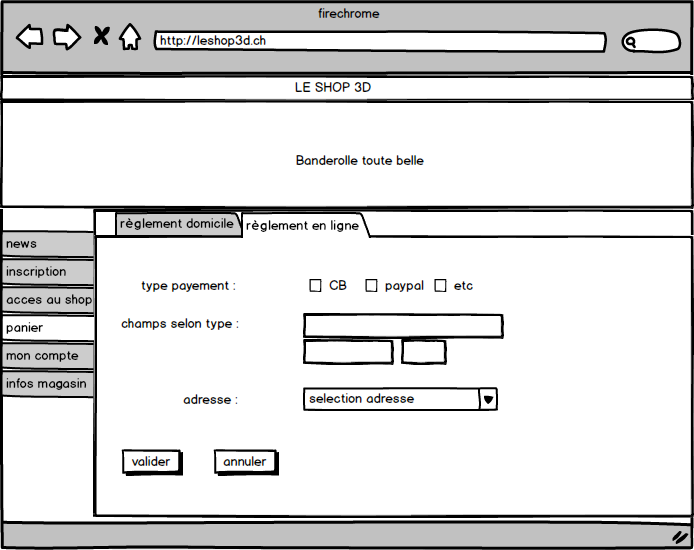
\includegraphics[scale=0.6]{../Maquettes/reglement_online.jpeg}
    \caption*{Règlement online}
\end{figure}

\newpage
\subsection{Navigation 3D}

\begin{figure}[ht]
    \center
    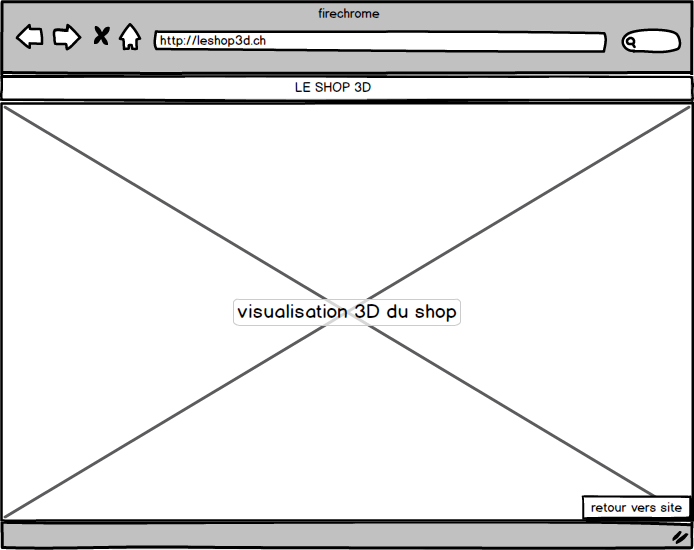
\includegraphics[scale=0.6]{../Maquettes/nav_3D.jpeg}
    \caption*{Navigation 3D du EShop}
\end{figure}

\newpage
\section{Architecture}
Nous avons décidé de développer l'application en utilisant WebGL (Front-end), PHP (Front+Back end) et MySQL (Database).
Le diagramme de composants ci-dessous montre le système complet.
\begin{figure}[ht]
    \center
    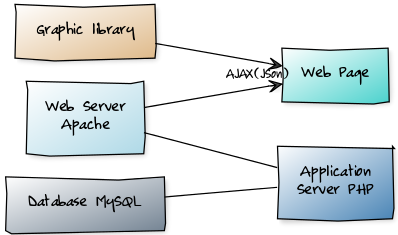
\includegraphics[scale=0.6]{../Diagrams/ComposantDiagrams/composants.png}
    \caption*{Diagramme UML de composants}
\end{figure}

\newpage
\section{Activités}

Voici les différents diagrammes d'activités de notre application.

\subsection{Recherche}

La recherche est accessible depuis le magasin 3D. Elle peut retourner soit une réponse positive,
avec le résultat de la recherche, soit aucun résultat, en revenant à la recherche.

\begin{figure}[ht]
    \center
    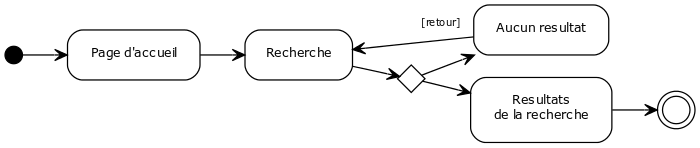
\includegraphics[scale=0.6]{../Diagrams/ActivityDiagrams/recherche.png}
    \caption*{Diagramme UML de la recherche d'un produit}
\end{figure}

\subsection{Gestion du panier}

Depuis le magasin 3D, on peut mettre un produit soit en allant le chercher directement dans le rayon,
soit en faisant une recherche pour un produit. Dès que l'on a trouvé un produit, on a la possibilité d'accéder
à sa description et de le mettre dans le panier.

\begin{figure}[ht]
    \center
    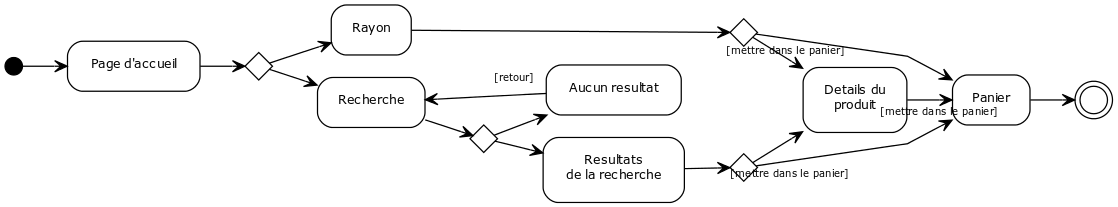
\includegraphics[scale=0.4]{../Diagrams/ActivityDiagrams/panier.png}
    \caption*{Diagramme UML de la gestion du panier}
\end{figure}

\newpage
\subsection{Commande d'un produit}

La commande d'un produit est accessible depuis la page de gestion de panier et
le paiement se fait par un intervenant externe.

\begin{figure}[ht]
    \center
    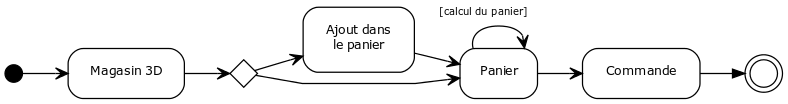
\includegraphics[scale=0.55]{../Diagrams/ActivityDiagrams/commande_global.png}
    \caption*{Diagramme UML de l'accès à la commande d'un produit}
\end{figure}

Pour pouvoir effectuer une commande, il faut être identifié.
Le client doit rentrer ses informations clients et de paiement.
A tout moment avant le paiement, le client peut annuler et retourner à la visualisation du panier.
La partie du paiment avec informations bancaires est externalisée.

\begin{figure}[ht]
    \center
    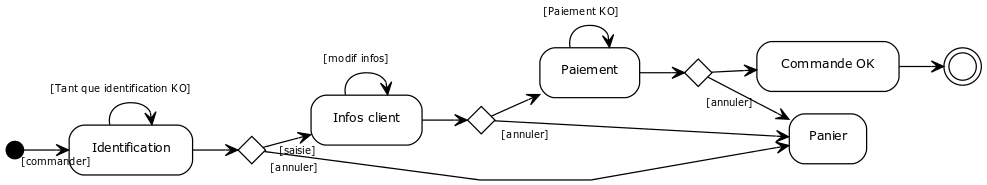
\includegraphics[scale=0.45]{../Diagrams/ActivityDiagrams/commande_en_cours.png}
    \caption*{Diagramme UML d'une commande}
\end{figure}

\newpage
\section{Séquences}

Voici les diagrammes de séquences de l'application.

\subsection{Recherche}

L'internaute peut faire la recherche d'un produit.
Celle-ci peut se terminer avec un échec s'il y a aucun résultat ou
avec un succès, en retournant les produits trouvés.
Il peut ensuite sélectionner les produits et avoir accès à leur description et
éventuellement les mettre dans le panier.

\begin{figure}[ht]
    \center
    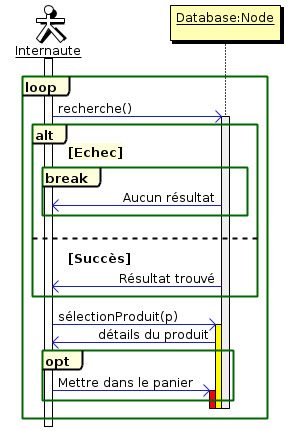
\includegraphics[scale=0.7]{../Diagrams/SequenceDiagrams/recherche.png}
    \caption*{Diagramme UML de la recherche d'un produit}
\end{figure}

\newpage
\subsection{Gestion du panier}

Après la recherche, l'utilisateur peut mettre les produits dans son panier.
Tant qu'il est sur l'affichage du panier, il peut modifier la quantité des produits et les supprimer de son panier.
Le panier est ensuite mis à jour.

\begin{figure}[ht]
    \center
    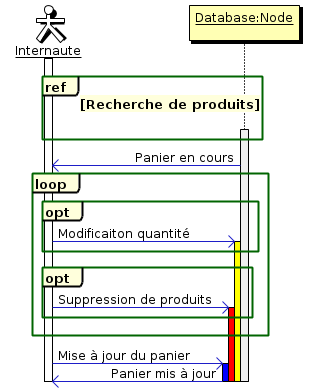
\includegraphics[scale=0.7]{../Diagrams/SequenceDiagrams/panier.png}
    \caption*{Diagramme UML de la gestion du panier}
\end{figure}

\newpage
\section{Modèle relationnel}

\begin{figure}[ht]
    \center
    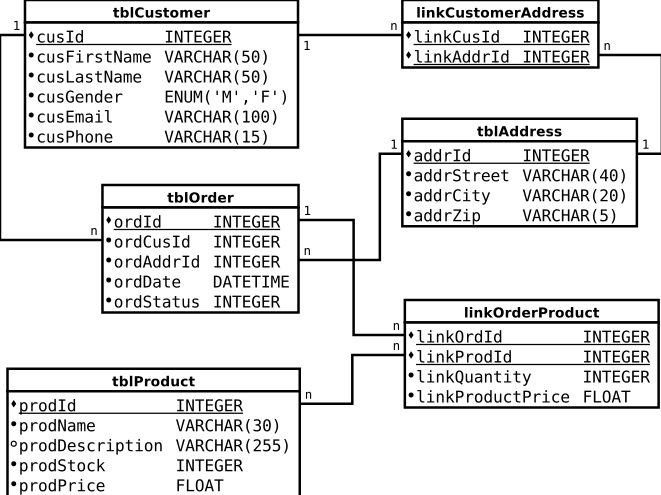
\includegraphics[scale=0.7]{../Diagrams/ClassDiagrams/Database.png}
    \caption*{Modèle relationnel de la base de donnée}
\end{figure}

\newpage
\section{Diagramme de classes}

\begin{figure}[ht]
    \center
    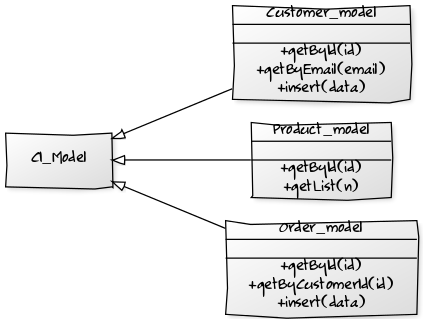
\includegraphics[scale=0.7]{../Diagrams/ClassDiagrams/Models.png}
    \caption*{Diagramme de classe de l'application}
\end{figure}

\newpage
\section{\textit{Sprints}}
Un sprint dure entre 2 et 4 semaines. Le deuxième semestre dure 8 semaines (sans compter les vacances de Pâques), donc nous avons décidé de prévoir 4 sprints.

\subsection{Sprint 1 - Architecture et 3D}
Dans ce sprint, on va mettre en place tout le système, développer le serveur PHP, très basique, et mettre en place la base données.
Notre but est de faire fonctionner le lien entre la partie 3D et la base de données.
À partir de ce moment là, nous passerons à la visualisation des produits stockés dans la base de données. Cette tâche répond au usecase de "Visualisation de produits".\\\\
Le deuxième usecase traité dans ce sprint est "Afficher la description d'un produit". Cela permettra de tester le fonctionnement de l'architecture mise en place.
A la fin du premier sprint, nous avons donc déjà un produit fonctionnel.

\subsection{Sprint 2 - Navigation, filtres et recherche}
Dans ce 2ème sprint, nous allons mettre en place la vue par catégories des produits, le filtre des produits et la recherche des produits.

\subsection{Sprint 3 - Panier}
Comme le titre du sprint l'indique, la gestion du panier se fera ici. Maintenant que l'utilisateur peut choisir ses produits en les filtrant, en naviguant
par catégories et faisant des recherches, il pourra après ce sprint, ajouter des produits dans son panier, modifier son panier et enfin accéder au système de paiement.
La partie de sélection de produit se faire via la 3D, mais toute la gestion se fera de manière classique.
Le système de paiement étant externe à notre logiciel, le client sera juste redirigé vers la page du site partenaire.
Le panier est géré par cookies, et donc la gestion des utilisateurs n'est pas requise à cette étape du projet.

\subsection{Sprint 4 - Utilisateurs}
Le dernier sprint n'est pas la partie la plus dure du projet, c'est pour cela qu'elle est à la fin.
Dans les comptes utilisateurs, nous pourrons stocker les adresses de facturation, les données clientes, et les informations de paiement.


\end{document}
